\documentclass[11pt]{article}
\usepackage[margin=0.8in]{geometry}
\usepackage{booktabs}
\usepackage{array}
\usepackage{xcolor}
\usepackage{pgfplots}
\usepackage{pgfplotstable}
\usepackage{tikz}
\usepackage{hyperref}
\usepackage{enumitem}
\usepackage{parskip}
\usepackage{makecell}

\pgfplotsset{compat=1.18}
\definecolor{siamdefault}{HTML}{8A5A44}
\definecolor{siamcal}{HTML}{C67C4E}
\definecolor{nnls}{HTML}{2A6F97}
\definecolor{deep}{HTML}{2F8F6B}
\definecolor{muted}{HTML}{555555}

\hypersetup{
  colorlinks=true,
  linkcolor=black,
  urlcolor=nnls
}

\title{\textbf{Mixture Classification Model Summary}\\
\large Raman mixtures, 17-class library, real-mixture evaluation}
\author{}
\date{\today}

\begin{document}
\maketitle

\section*{Executive Summary}

The original mixture-classification approach used a two-head Siamese network: one head processed the standard Raman spectrum, the other processed a Fourier/FFT representation, and a multilabel MLP predicted which chemicals were present. That model was useful for early exploration, but after expanding the library to 17 possible chemicals it did not handle the larger decision space well. It tended to return too many chemicals per sample and therefore had low exact-match performance.

Two newer approaches are substantially stronger on the actual measured mixture task. The best classical model is a \textbf{Replicate-Dictionary Pair NNLS} method. The best deep model is a \textbf{Similarity-Supervised Coefficient Regressor}. Both are evaluated on real mixture spectra only: 580 original real mixtures plus 324 PT2 real mixtures, for 904 total measured mixture spectra. Pure spectra and synthetic spectra are not included in the tables below.

\section*{What Was Tested}

All models are evaluated in the same 17-class chemical library. The final task is binary mixture identification: each real mixture contains two chemicals, and a prediction is exactly correct only if both chemicals are recovered and no extras are returned.

\begin{center}
\begin{tabular}{p{0.24\linewidth}p{0.68\linewidth}}
\toprule
\textbf{Model} & \textbf{Interpretation} \\
\midrule
Siamese+MLP 2-head & Original model. Encodes Raman and FFT views, then predicts each chemical independently with thresholds. \\
Replicate-Dictionary Pair NNLS & Classical unmixing model. Searches all possible binary pairs and chooses the pair whose reference spectra best reconstruct the measured mixture. \\
Similarity-Supervised Coefficient Regressor & Deep coefficient model. Learns to map a mixture spectrum to nonnegative chemical shares over all 17 compounds, then returns the top two. \\
\bottomrule
\end{tabular}
\end{center}

\section*{Main Results}

\begin{center}
\begin{tabular}{lrrrrr}
\toprule
\textbf{Model} & \textbf{Exact} & \textbf{Precision} & \textbf{Recall} & \textbf{F1} & \textbf{Avg. returned} \\
\midrule
Siamese+MLP default 0.5 & 0.306 & 0.614 & 0.887 & 0.726 & 2.889 \\
Siamese+MLP calibrated & 0.301 & 0.572 & 0.905 & 0.701 & 3.166 \\
Replicate-Dictionary Pair NNLS & 0.940 & 0.970 & 0.970 & 0.970 & 2.000 \\
Similarity-Supervised Coefficient Regressor & 0.969 & 0.983 & 0.983 & 0.983 & 2.000 \\
\bottomrule
\end{tabular}
\end{center}

\begin{figure}[ht]
\centering
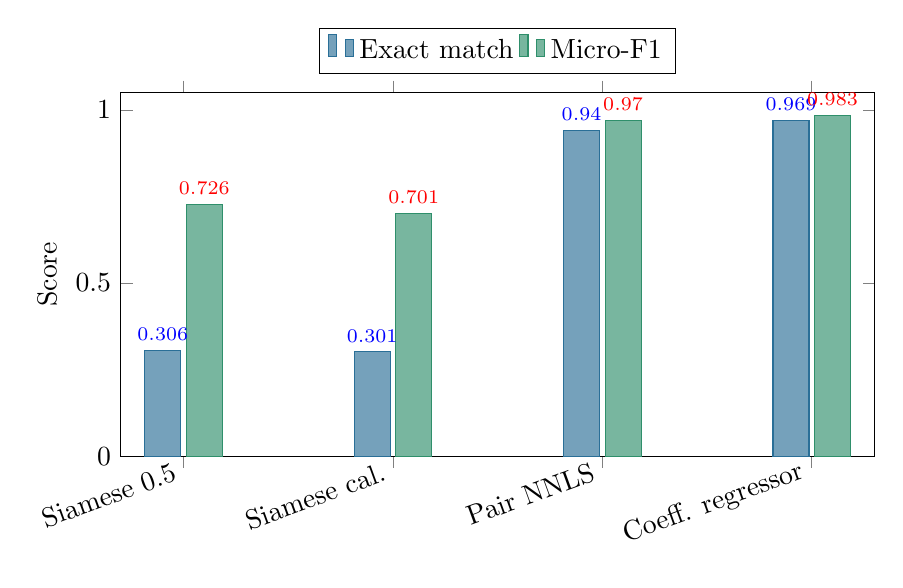
\begin{tikzpicture}
\begin{axis}[
  ybar,
  width=0.92\linewidth,
  height=6.2cm,
  ymin=0,
  ymax=1.05,
  ylabel={Score},
  symbolic x coords={Siamese 0.5,Siamese cal.,Pair NNLS,Coeff. regressor},
  xtick=data,
  x tick label style={rotate=20,anchor=east},
  bar width=13pt,
  legend style={at={(0.5,1.05)},anchor=south,legend columns=2},
  nodes near coords,
  nodes near coords style={font=\scriptsize,/pgf/number format/fixed,/pgf/number format/precision=3},
]
\addplot+[fill=nnls!65,draw=nnls] coordinates {
  (Siamese 0.5,0.306) (Siamese cal.,0.301) (Pair NNLS,0.940) (Coeff. regressor,0.969)
};
\addplot+[fill=deep!65,draw=deep] coordinates {
  (Siamese 0.5,0.726) (Siamese cal.,0.701) (Pair NNLS,0.970) (Coeff. regressor,0.983)
};
\legend{Exact match,Micro-F1}
\end{axis}
\end{tikzpicture}
\caption{Exact match requires both mixture chemicals to be correct. Micro-F1 measures chemical-level precision and recall. The two newer models are much stronger than the original Siamese pipeline on both metrics.}
\end{figure}

\begin{figure}[ht]
\centering
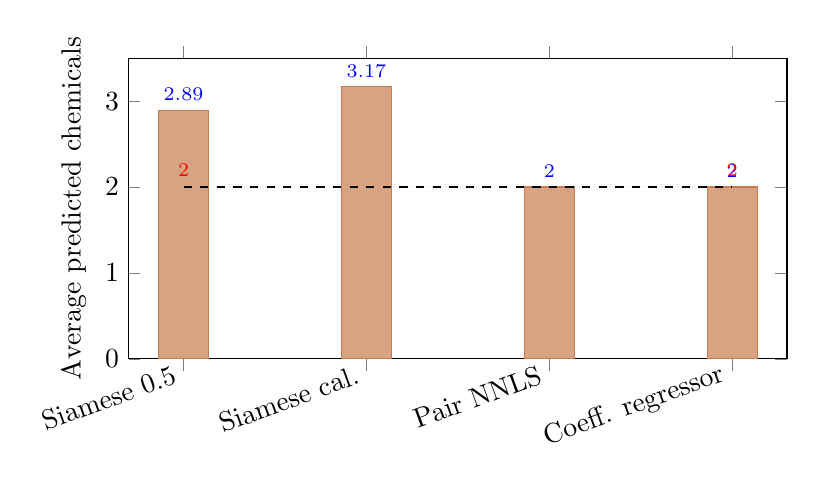
\begin{tikzpicture}
\begin{axis}[
  ybar,
  width=0.82\linewidth,
  height=5.4cm,
  ymin=0,
  ymax=3.5,
  ylabel={Average predicted chemicals},
  symbolic x coords={Siamese 0.5,Siamese cal.,Pair NNLS,Coeff. regressor},
  xtick=data,
  x tick label style={rotate=20,anchor=east},
  bar width=18pt,
  nodes near coords,
  nodes near coords style={font=\scriptsize,/pgf/number format/fixed,/pgf/number format/precision=2},
]
\addplot+[fill=siamcal!70,draw=siamcal] coordinates {
  (Siamese 0.5,2.889) (Siamese cal.,3.166) (Pair NNLS,2.000) (Coeff. regressor,2.000)
};
\addplot+[sharp plot,thick,draw=black,dashed] coordinates {
  (Siamese 0.5,2.000) (Coeff. regressor,2.000)
};
\end{axis}
\end{tikzpicture}
\caption{The real mixtures contain exactly two chemicals. The Siamese models over-return chemicals, while the pair NNLS and coefficient regressor return exactly two by design.}
\end{figure}

\section*{How The Original Siamese+MLP Model Works}

The original model has two feature-extraction heads. One Siamese encoder sees the baseline-processed Raman spectrum, and the second Siamese encoder sees a Fourier/FFT representation. Their embeddings are concatenated and sent to a multilabel MLP with one output per chemical.

This means each chemical is decided independently: if the output score for a chemical is above a threshold, that chemical is returned. The default model uses a threshold of 0.5 for every chemical. The calibrated model uses class-specific thresholds learned from an earlier calibration run. Calibration improved some individual recalls, but it also increased false positives. That is why the calibrated model returns about 3.17 chemicals per sample on average even though the true mixtures have exactly two.

\section*{Replicate-Dictionary Pair NNLS}

\subsection*{Standard Pair NNLS}

Standard pair NNLS is a classical unmixing method. For each possible chemical pair, it asks: can a nonnegative combination of the two reference spectra reconstruct the measured mixture? It solves a nonnegative least-squares fit for every pair and returns the pair with the smallest residual.

This is a strong starting point because Raman mixtures are often close to additive: the observed spectrum can often be approximated as a weighted sum of pure spectra. It also matches the binary mixture structure directly.

\subsection*{What The Replicate Dictionary Adds}

The selected classical model improves on standard pair NNLS by changing how each chemical is represented. Instead of one reference spectrum per compound, each compound gets a small dictionary:

\begin{itemize}[leftmargin=*]
\item the mean spectrum for that compound;
\item up to nine representative replicate spectra selected to cover within-class variation;
\item one shared constant baseline atom to absorb simple background offset.
\end{itemize}

At inference time, the model still searches all possible binary pairs. For a candidate pair, it combines both compounds' replicate dictionaries and the baseline atom into one design matrix. It then solves NNLS and records the residual. The predicted chemicals are the pair with the lowest residual.

The important point is that this model is not trained on labeled mixtures. It is built from the pure reference library, then evaluated on real mixtures. Its strength comes from a physically meaningful constraint: a valid answer should reconstruct the measured spectrum using nonnegative amounts of two library compounds.

\begin{figure}[ht]
\centering
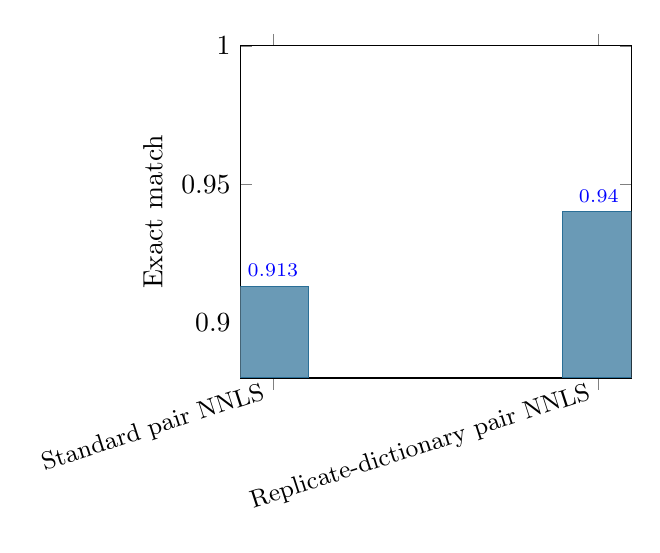
\begin{tikzpicture}
\begin{axis}[
  ybar,
  width=0.54\linewidth,
  height=5.8cm,
  ymin=0.88,
  ymax=1.00,
  ylabel={Exact match},
  symbolic x coords={Standard pair NNLS,Replicate-dictionary pair NNLS},
  xtick=data,
  x tick label style={rotate=18,anchor=east,font=\small},
  bar width=26pt,
  nodes near coords,
  nodes near coords style={font=\scriptsize,/pgf/number format/fixed,/pgf/number format/precision=3},
]
\addplot+[fill=nnls!70,draw=nnls] coordinates {
  (Standard pair NNLS,0.913)
  (Replicate-dictionary pair NNLS,0.940)
};
\end{axis}
\end{tikzpicture}
\caption{Focused classical comparison on the same 904 real-mixture spectra. The replicate dictionary improves standard pair NNLS by representing each compound with multiple reference atoms rather than one prototype.}
\end{figure}

\section*{Similarity-Supervised Coefficient Regressor}

\subsection*{Standard Coefficient Regressor}

The standard coefficient regressor is a deep model, but its output is still interpretable. It takes one preprocessed spectrum and predicts 17 nonnegative coefficient shares, one per chemical. The shares are normalized to sum to one. At inference time, the two largest shares are returned as the predicted mixture components.

This differs from the Siamese+MLP model. The Siamese model asks 17 independent yes/no questions. The coefficient regressor asks a constrained allocation question: how should one unit of chemical contribution be distributed across the 17 library compounds?

It is helpful to think of coefficient regression as the deep-learning analogue of NNLS. NNLS solves a fresh optimization problem for each new spectrum: find nonnegative coefficients that best reconstruct the measured spectrum from the reference dictionary. The coefficient regressor learns a direct function from spectrum to coefficients during training. At deployment time it does not solve an optimization problem; it uses one neural-network forward pass to estimate the coefficient vector. So both methods are trying to recover nonnegative chemical contributions, but NNLS solves them per sample while the regressor learns to predict them.

\subsection*{How It Is Trained}

The deep model is trained on synthetic binary mixtures made from pure reference spectra. For every chemical pair, mixtures are generated at ratios from 0.1 to 0.9. Random replicate spectra are sampled, global intensity scaling is applied, and small Gaussian noise is added. These synthetic spectra are split into train, validation, and test sets for internal model selection.

The final results in this report are not synthetic-test results. After training, the model is evaluated on the 904 measured real mixture spectra.

\begin{center}
\begin{tabular}{p{0.30\linewidth}p{0.60\linewidth}}
\toprule
\textbf{Component} & \textbf{Protocol} \\
\midrule
Input & Baseline-corrected Raman spectrum, normalized before the neural-network forward pass. \\
Architecture & Fully connected MLP: input $\rightarrow$ 512 units + layer normalization + GELU + dropout; 512 $\rightarrow$ 256 units + layer normalization + GELU + dropout; 256 $\rightarrow$ 17 output logits. \\
Output constraint & Softplus makes outputs nonnegative; outputs are divided by their sum to produce 17 coefficient shares that sum to one. \\
Synthetic training data & Binary mixtures generated from pure reference spectra for every pair of the 17 chemicals. This produces 12,240 synthetic spectra total: 136 chemical pairs $\times$ 9 ratios $\times$ 10 random draws. The stratified split uses 9,792 spectra for gradient training, 1,224 for validation, and 1,224 for synthetic test audit. \\
Augmentation & Random reference replicates, random global scale from 0.85 to 1.15, and small Gaussian noise. \\
Model selection & Synthetic train/validation/test split stratified by chemical pair. Real mixtures are reserved for final evaluation. \\
Inference rule & Rank the 17 predicted shares and return the top two chemicals. \\
\bottomrule
\end{tabular}
\end{center}

\subsection*{What Similarity Supervision Adds}

The similarity-supervised version keeps the same coefficient-regression idea but adds losses that make the ranking more robust:

\begin{itemize}[leftmargin=*]
\item coefficient loss: predicted shares should match the synthetic mixture ratios;
\item support loss: true chemicals should score above inactive chemicals;
\item reconstruction loss: predicted shares should reconstruct the spectrum through a fixed reference dictionary;
\item margin-ranking loss: the weakest true chemical should stay above the strongest false chemical;
\item similarity-weighted false-positive loss: false positives are penalized more when they are spectrally similar to the true chemicals.
\end{itemize}

That last term is the key difference from the standard coefficient regressor. It teaches the model that confusing a true chemical with a very similar impostor is especially costly. This is useful for chemically similar families where residual-based classical fitting can produce near ties.

\begin{figure}[ht]
\centering
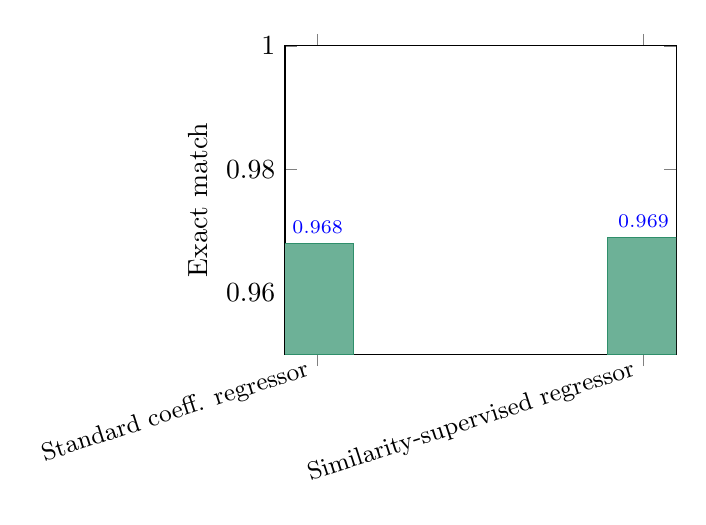
\begin{tikzpicture}
\begin{axis}[
  ybar,
  width=0.54\linewidth,
  height=5.5cm,
  ymin=0.95,
  ymax=1.00,
  ylabel={Exact match},
  symbolic x coords={Standard coeff. regressor,Similarity-supervised regressor},
  xtick=data,
  x tick label style={rotate=18,anchor=east,font=\small},
  bar width=26pt,
  nodes near coords,
  nodes near coords style={font=\scriptsize,/pgf/number format/fixed,/pgf/number format/precision=3},
]
\addplot+[fill=deep!70,draw=deep] coordinates {
  (Standard coeff. regressor,0.968)
  (Similarity-supervised regressor,0.969)
};
\end{axis}
\end{tikzpicture}
\caption{Focused deep comparison on the same 904 real-mixture spectra. The similarity-supervised coefficient regressor is slightly ahead of the standard coefficient regressor while preserving the same top-two inference rule.}
\end{figure}

\section*{How To Interpret The Results}

Exact match is the strictest metric. A prediction is counted correct only if both chemicals are right and no extra chemical is returned. This is the most relevant metric because the mixtures are binary.

Micro-F1 is a chemical-level metric. It gives partial credit when one of the two chemicals is correct, but the other is missed or an extra chemical is predicted. This is useful diagnostically, but exact match is easier to interpret operationally.

The key result is that the two newer models both enforce the binary structure of the task at inference time. They return exactly two chemicals per measured mixture. The original Siamese+MLP model does not enforce this and overpredicts, especially after calibration.

\section*{Conclusion}

The initial two-head Siamese+MLP model did not scale cleanly when the library expanded to 17 chemicals. The stronger current baselines are better aligned with the mixture problem. The replicate-dictionary pair NNLS model works because it directly fits each measured spectrum against all possible binary supports using real reference spectra. The similarity-supervised coefficient regressor works because it learns a global 17-class coefficient ranking while still returning the top two chemicals at inference.

On the final real-mixture benchmark, the similarity-supervised coefficient regressor is the best clean model, with exact match 0.969 and micro-F1 0.983. The replicate-dictionary pair NNLS model remains a strong non-deep baseline, with exact match 0.940 and micro-F1 0.970.

\section*{Bonus: Inference Speed}

The coefficient regressor is much faster at deployment time because training has already amortized the unmixing work. Replicate-dictionary NNLS solves a fresh optimization problem for every candidate pair and every new spectrum. The coefficient regressor performs matrix multiplications in a trained neural network and returns the top two shares.

The timing experiment used the same 904 measured mixture spectra and excluded data loading and deep-model training. The CPU-only benchmark is the fairest comparison because both methods run without GPU acceleration. On this benchmark, single-spectrum coefficient-regressor inference is about \textbf{118 times faster} than replicate-dictionary NNLS. When all 904 spectra are processed as one batch, the regressor is about \textbf{4,570 times faster per spectrum}; the full dataset takes about 1.7 milliseconds instead of 7.7 seconds.

\begin{center}
\begin{tabular}{p{0.32\linewidth}p{0.23\linewidth}rrr}
\toprule
\textbf{Method} & \textbf{Inference mode} & \textbf{Total time} & \textbf{ms/sample} & \textbf{Speedup} \\
\midrule
Replicate-Dictionary Pair NNLS & Per-spectrum exhaustive pair search & 7.687 s & 8.504 & 1.0$\times$ \\
Similarity-Supervised Coefficient Regressor & Single-spectrum loop & 0.0654 s & 0.0723 & 117.6$\times$ \\
Similarity-Supervised Coefficient Regressor & Batched forward pass & 0.00168 s & 0.00186 & 4569$\times$ \\
\bottomrule
\end{tabular}
\end{center}

\begin{figure}[ht]
\centering
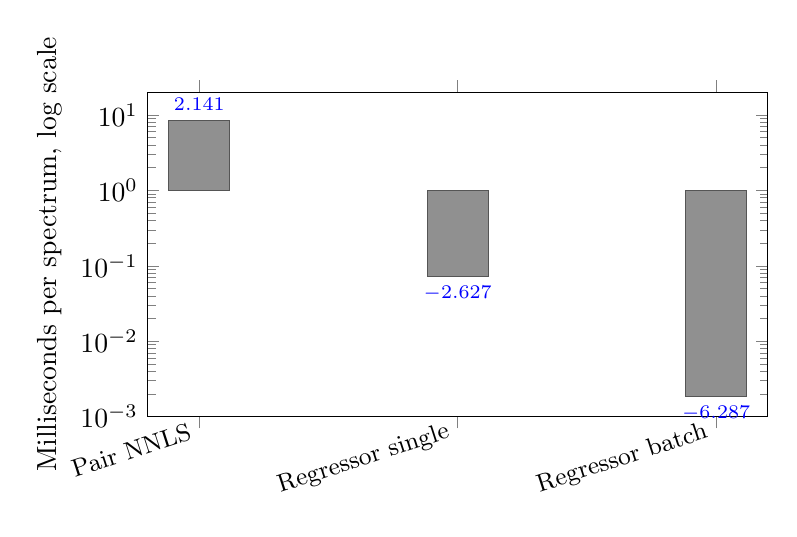
\begin{tikzpicture}
\begin{axis}[
  ybar,
  ymode=log,
  width=0.78\linewidth,
  height=5.7cm,
  ylabel={Milliseconds per spectrum, log scale},
  symbolic x coords={Pair NNLS,Regressor single,Regressor batch},
  xtick=data,
  x tick label style={rotate=18,anchor=east,font=\small},
  bar width=22pt,
  ymin=0.001,
  ymax=20,
  nodes near coords,
  nodes near coords style={font=\scriptsize,/pgf/number format/fixed,/pgf/number format/precision=3},
]
\addplot+[fill=muted!65,draw=muted] coordinates {
  (Pair NNLS,8.504)
  (Regressor single,0.0723)
  (Regressor batch,0.00186)
};
\end{axis}
\end{tikzpicture}
\caption{CPU-only inference timing. The coefficient regressor is about 118 times faster than replicate-dictionary NNLS when run one spectrum at a time, and about 4,570 times faster per spectrum when batched.}
\end{figure}

\end{document}
